%%%%%%%%%%%%%%%%%%%%%%%%%%%%%%%
%   Figures for chapter 4
%%%%%%%%%%%%%%%%%%%%%%%%%%%%%%%

\newcommand{\figFrameworkFlow}{
    \begin{figure}
        \centering
        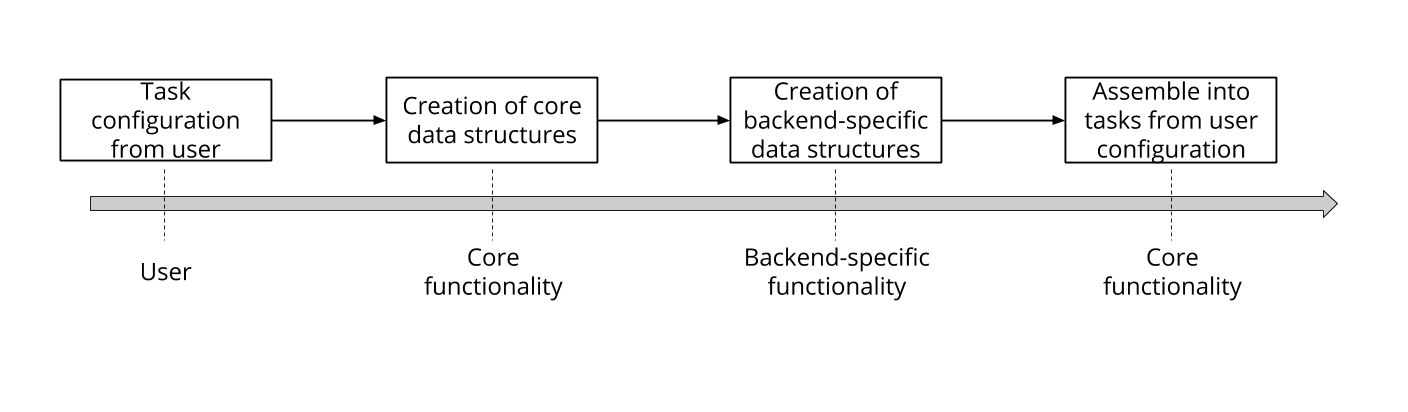
\includegraphics[width=0.9\textwidth]{./chapters/chapter_4/imgs/img_ch4_framework_flow.png}
        \caption{Flow of data in the proposed framework}
        \label{fig:ch4_proposed_framework_flow}
    \end{figure}
}

\newcommand{\figFrameworkArchitecture}{
    \begin{figure}
        \centering
        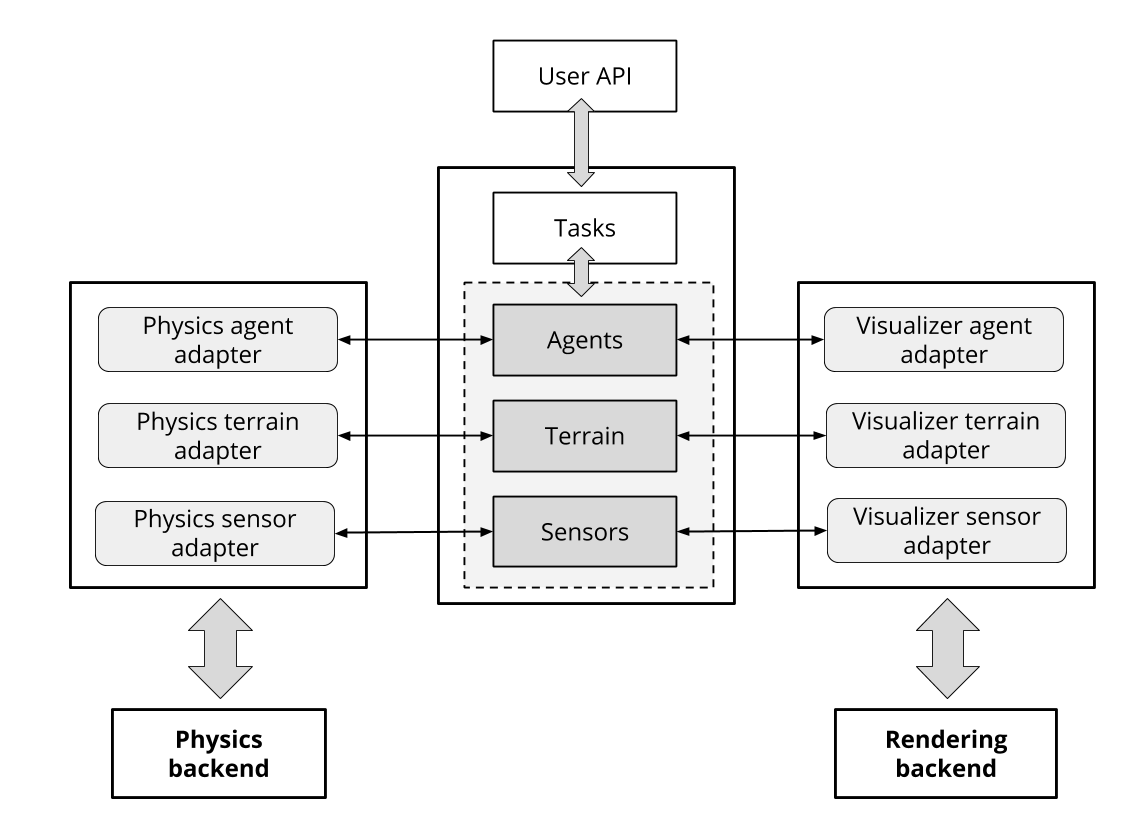
\includegraphics[width=0.9\textwidth]{./chapters/chapter_4/imgs/img_ch4_framework_architecture.png}
        \caption{Architecture of the proposed framework}
        \label{fig:ch4_proposed_framework_architecture}
    \end{figure}
}

\newcommand{\figFrameworkCoreAgent}{
    \begin{figure}[!ht]
        \centering
        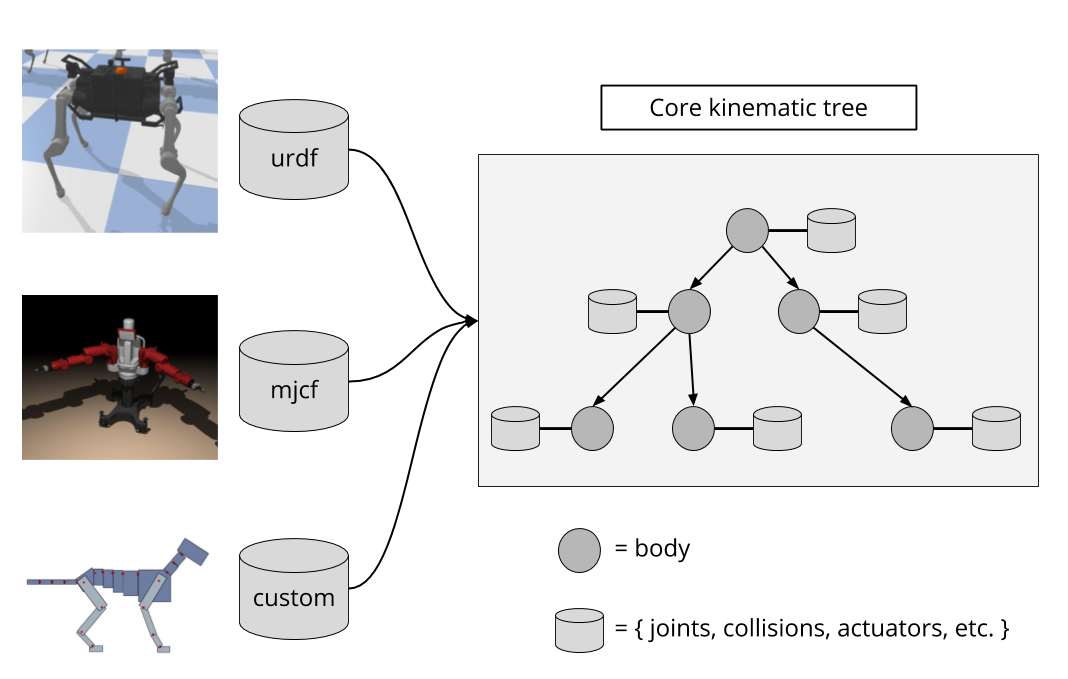
\includegraphics[width=0.9\textwidth]{./chapters/chapter_4/imgs/img_ch4_agents_core.png}
        \caption{Core agent functionality. Model formats are loaded into 
                 the core kinematic tree}
        \label{fig:ch4_core_agent_functionality}
    \end{figure}
}

\newcommand{\figFrameworkCoreTerrain}{
    \begin{figure}[!ht]
        \centering
        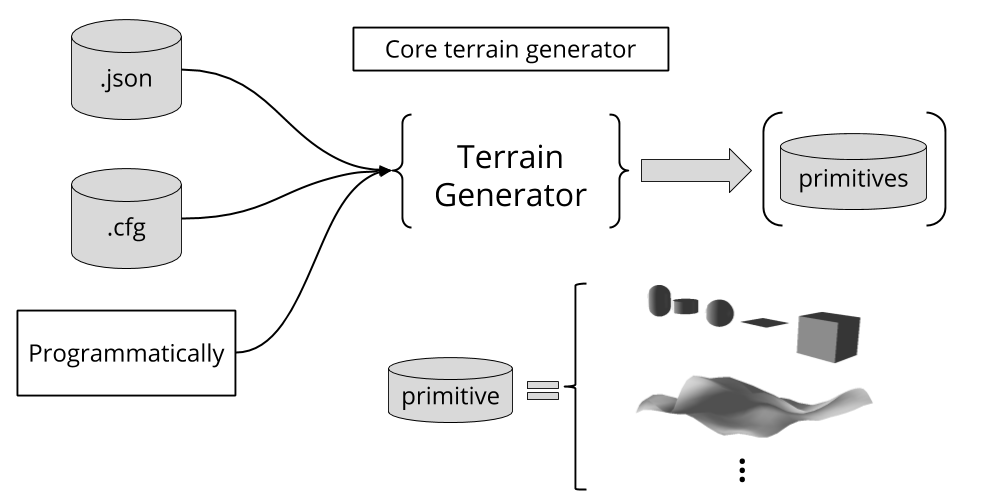
\includegraphics[width=0.9\textwidth]{./chapters/chapter_4/imgs/img_ch4_terrain_core.png}
        \caption{Core terrain functionality. User configuration is passed to the terrain generator
                 and the generator then creates blueprints to be used by the backend.}
        \label{fig:ch4_core_terrain_functionality}
    \end{figure}
}

\newcommand{\figFrameworkCoreSensor}{
    \begin{figure}[!ht]
        \centering
        \begin{subfigure}[b]{0.3\textwidth}
            \centering
            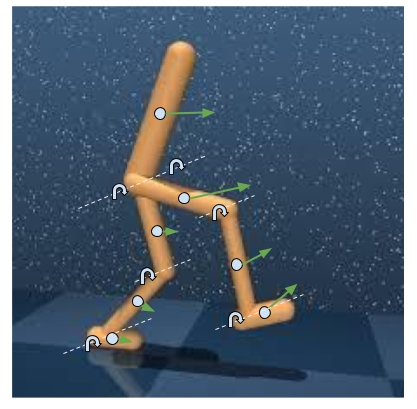
\includegraphics[width=0.9\textwidth]{./chapters/chapter_4/imgs/img_ch4_sensors_core_1.png}
            \caption{}
            \label{fig:ch4_core_sensor_1}
        \end{subfigure}
        \begin{subfigure}[b]{0.3\textwidth}
            \centering
            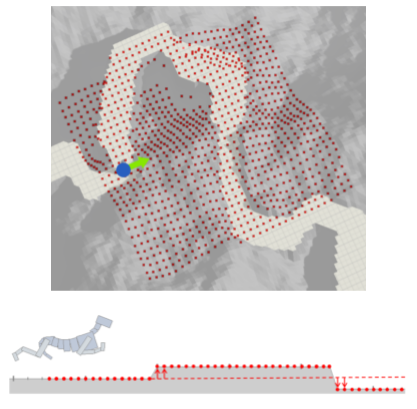
\includegraphics[width=0.9\textwidth]{./chapters/chapter_4/imgs/img_ch4_sensors_core_2.png}
            \caption{}
            \label{fig:ch4_core_sensor_2}
        \end{subfigure}
        \begin{subfigure}[b]{0.3\textwidth}
            \centering
            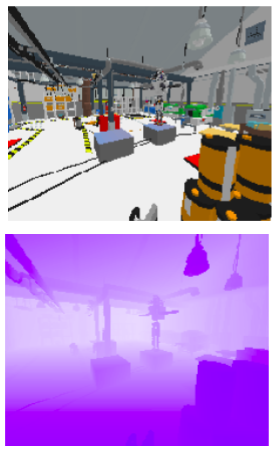
\includegraphics[width=0.9\textwidth]{./chapters/chapter_4/imgs/img_ch4_sensors_core_3.png}
            \caption{}
            \label{fig:ch4_core_sensor_3}
        \end{subfigure}
        \caption{Core sensors functionality. a) Intrinsic readings from joints and bodies (adapted from [@CITE]).
                                             b) Extrinsic readings from heightmaps of the terrain (adapted from [@CITE,@CITE]).
                                             c) Extrinsic readings from rgb and depth images of the agent view (adapted from [@CITE]).}
        \label{fig:ch4_core_sensor_functionality}
    \end{figure}
}

\newcommand{\figBridgePattern}{
    \begin{figure}
        \centering
        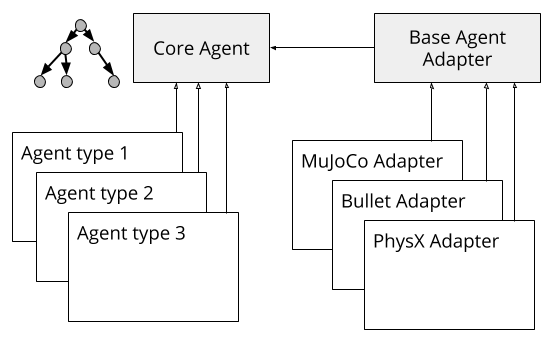
\includegraphics[width=0.8\textwidth]{./chapters/chapter_4/imgs/img_ch4_bridge_pattern.png}
        \caption{Bridge pattern used to decouple agent functionality}
        \label{fig:ch4_bridge_pattern}
    \end{figure}
}